\documentclass[11pt]{article}

\usepackage[top=0.6in, bottom=0.6in, left=0.5in, right=0.5in]{geometry} 
\usepackage{graphicx}
\usepackage{url}
\usepackage{indentfirst}

\begin{document}

\title{Profiling Analysis of the Box2D Simulation}

\author{Pratik Fegade 120050004\\
Krishna Deepak 120050057\\
Bharath Kumar 120050058\\}
\maketitle

\section{Introduction}
This report is our analysis of the timing data of the Box2D simulation obtained by using various utilities like gettimeofday(), the time command line utility and the profilers gprof and perf. Sections of the code that take up a significant amount of time to execute are identified and thus are they can be optimised further to reduce the running time of the simulation.

\section{Analysis of the Looptime and Related Data}

\subsection{Analysis of the Data}
The data is obtained by running the simulation for some reruns for a particular number of steps and averaging over the reruns. Data for looptime, steptime, time required for position, collision and velocity updates was collected. The steptime is significantly high for low number of iterations (probably due to all the variable initializations required at the start of the simulation) and it falls quickly and stabilises. Similar but less pronounced effects are seem with the times required for velocity, postion and collision updates. Also the sum of the average times required for velocity, postion and collision updates signoficantly falls short of the average steptime suggesting that some other not examined function takes up significant amounts of time. For all the iteration values, the velocity update time is the highest while the collision update time is the lowest. A plot of these average times is shown below.
\\
\begin{center}
	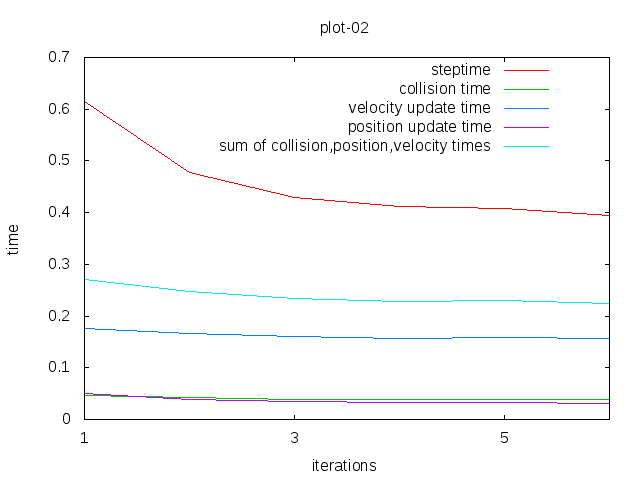
\includegraphics[width=12cm]{./images/g04_plot02.png}
\end{center}
\indent The average steptime for a significant number of iterations is almost stable though it sometimes varies a lot over the reruns. This is demonstrated by plotting a frequency plot of the steptimes over the reruns for a particular value of the number of iterations (58 in our case). The plot as expected shows a concentrations of stetimes around the average steptime but it does have a significant tail as a result of some high values of the steptime.
\\
\indent The data was generated for 150 reruns for each iteration (1 to 1500). However, a plot of the line obtained by applying linear regression on  average steptime of randomly selected 15 reruns out of the 150 reruns shows stiking similarity to that obtained by regressing over the entire data. Hence it seems that the analysis would not differ much even if data is collected for a smaller number of reruns.

\subsection{Effect of CPU/Memory Load on the Data}
\indent The data depends on the memory and the cpu load on the machine the simulation is being run on. The average times show a noticeable rise when the cpu is loaded with other processor intensive processes. The graph below plots the average times obtained with a loaded cpu. 
\\
\begin{center}
	\includegraphics[width=12cm]{./images/proc_g04_plot02.png}
\end{center}
The times in the case when there is a significant load on the memory are lesser than the case when the processor is loaded however are still higher than the case when the system is not loaded in the case of the memory or the processor. This is because the simulation is not as memory intensive as it is processor intensive.
\\
\indent The command line utility time gives 3 different times - real, user and sys times. The user time corresponds to actual time elapsed. The user time gives the time spent by the process that time is invoked on on the cpu while the system time gives the time the OS takes to perform tasks for the process. The real time thus can be affected by other processes running as it is the actual time interval. On invoking the time utility on the simulation it is observed that the looptime is smaller than the user time, which in turn is smaller than the real time. Also the system time is very low are compared to the other times. The looptime is smaller than the user time as the simulation does other tasks (initialisations and related tasks like setting up standard utilities like stdin and stdout)\cite{startOfCppprog} apart from just running the loop.


\section{Analysis of Profiling Data}
The profiling data for the simulation was generated by running it for 50,000 steps for 3 reruns. Most of the functions in the simulation source code should have been called and hence profiled as the simulation was run for 50,000 steps. The profiler perf\cite{perfsite} was used to generate the data. Following is analysis of the data of both the release and the debug builds of the simulation and a comparison of both.

\subsection{Analysis of the Release Build}
 In the case of the release build, the b2ContactSolver::SolveVelocityConstraints() function takes the maximum amount of time (about 30\% of the total) amongst all the functions profiled. This is followed by the b2World::Solve function and the b2ContactSolver::SolvePositionConstraints() function. This is consistent with the observations made from the timing data analysed above as there too, the velocity update time was the higher than the position and collision update times. We ignore the functions that are not in the simulation code and are a part of some libraries (these hence include the GLUT, GLUI, OpenGL and any functions that are a part of any standard C++ or system libraries).

\subsection{Analysis of the Debug Build}
We have run the base code for 50000 iterations, 3 reruns and profiled the code using perf.
Excluding the functions related to GLUI or GLUT, b2ContactSolver::SolveVelocityConstraints() took the most percentage of time(about 22\%) in all the 3 reruns. Following it, there are functions which perform operations *,-,+ which took  maximum amount of time. b2ContactSolver::SolveVelocityConstraints() takes more time than b2ContactSolver::SolvePositionConstraints(). This observation is consistent with the observations made in the 'Analysis of Release Build' and 'Analysis of the Looptime and Related Data'. Following it, there are functions relating to Collisions, Joints, Body, Vectors etc.
\\
\\
\indent In both the above cases, as the number of iterations the simulation is run for rises, the time taken by b2ContactSolver::SolveVelocityConstraints() relative to the total time remains almost constant. Similar is the case with the other functions that take significant amount of time. For a smaller number of iterations some functions in  libraries like [kernel.kallsyms] take a large portion of the total running time. However this is not observed with large number of iteraions probably because they take a constant amount of tme to execute indepedent of the number of the iteartions.
\subsection{A Comparison of Debug and Release Data}
The profile generated for the debug build is significantly larger than the one for the release build (compiled with level 3 optimization). This makes the debug profile much more informative and fine-grained and hence easier for debugging the code. The debug profile most significantly contains the overhead data for all the operators defined for the various structs (vectors and similar objects) used in the simulation. Also, it includes the data for the constructors and destructors of the classes. It turns out that these do consume a significant amount of the total time. This critical information is not however, accounted for in the release version profile.
\\
\indent The -03 or -o2 options given to g++ during compilation tell the compiler to optimize the code to a desired level (2 or 3 in this case). The profiler can generate so much more information in the case of the debug build as the compiler consider statements as independent and hence does not optimize the code when complied in the debug mode. As a result the functions which the compiler would normally optimize (like constructors, destructors and operators) are left as they are and hence the compiler can then insert appropriate debug symbols for each of these functions (and hence the debug build is significantly larger than the release build) thus enabling the profiler to gather data about these functions. In the release build the compiler highly optimizes the code and all the functions it optimizes are unobservable as far as the profiler is concerned\cite{comp_optim}.
\\
\indent As the both the release and the debug profiles suggest, the b2ContactSolver::SolveVelocityConstraints() function is the one that if improved/optimised would lead to faster simulations. Also, as is evident from the debug profile, the operators - especially operator\*(float, b2Vec2 const\&) and operator\-(b2Vec2 const\&, b2Vec2 const\&) are used often and hence an improvement in their implementations would affect the performnace of the simulation. Also, one might try to reduce the number of calls to these operators/functions by some means.
\\
\begin{center}
	\includegraphics[height=25.5cm]{./images/output.png}
\end{center}
\subsection{The Call Graph}
The call graph generated for the debug build by perf is shown on the previous page. As the call graph shows, the execution of the C++ code starts with the execution of \_\_libc\_start\_main in the library libc-2.17.so which later calls the main function of the simulation. Also, it is seen that most of the functions execute within a reasonable amount of time and that only some functions take an extraordinarily large amount of time.

\bibliographystyle{plain}
\bibliography{g04_prof_report_ref.bib}

\end{document}
